\documentclass[12pt]{article}
\usepackage{geometry}
\geometry{a4paper, margin=2cm}
\topmargin = -50pt
\textheight = 24cm
\footskip = 50pt

\usepackage{polski}
\usepackage{libertine}
\usepackage[T1]{fontenc}
\usepackage[utf8]{inputenc}

\usepackage{indentfirst}
\usepackage{graphicx}
\usepackage{amsmath}
\usepackage{float}
\usepackage{multirow}
\usepackage{enumitem}
\usepackage[version=4]{mhchem}
\usepackage{chemfig}
\usepackage{amssymb}
\usepackage{caption}
\captionsetup[figure]{skip=-15pt}


\title{Wyznaczanie stechiometrii kompleksu}
\author{Kamila Wojdyna}
\date{14.03.2023r.}


\begin{document}

\maketitle


\begin{abstract}
    Do wyznaczenia stechiometrii kompleksu utworzonego z~jonów żelaza(II) oraz \textit{o}--fenantroliny wykorzystano metodę zmian ciągłych oraz metodę stosunków molowych. Metoda zmian ciągłych pozwoliła uzyskać wyniki stwierdzające, że stosunek jonów żelaza(II) do \textit{o}--fenantroliny wynosi 1:4 lub 1:3. W~ramach metody stosunków molowych uzyskano punkty pomiarowe, które nie układały się liniowo. Stąd część punktów została odrzucona, uzyskując proste przecinające się dla stosunku molowwego 1:3, co odpowiada rzeczywistej stechiometrii kompleksu. Ostatecznie otrzymano wyniki spójne, choć niejednoznaczne. Jako przyczynę podejrzewa się stężenia roztworów inne od zakładanych oraz niską wartość pH równą 2,40, która mogła wpływać na tworzenie się kompleksu.
\end{abstract}


\section{Cel doświadczenia}

Wyznaczenie stechiometrii związku kompleksowego utworzonego z~jonów żelaza(II) oraz \textit{o}--fenantroniny, poprzez zastosowanie metody zmian ciągłych oraz metody stosunków molowych.



\section{Wprowadzenie}

Stechiometria związków kompleksowych może zostać wyznaczona eksperymentalnie. Wśród sposobów pozwalających to uczynić można wymienić metodę zmian ciągłych oraz metodę stosunków molowych. Poniżej opisano te dwie metody przy założeniu, że związek kompleksowy jest złożony ze składnika A oraz składnika B, przy czym jego tworzenie jest opisane poniższym równaniem reakcji:

\begin{center}
    \ce{i A + j B <--> A_iB_j}
\end{center}



Metoda zmian ciągłych, znana też jako metoda Job'a, wykorzystuje
roztwory różniące się między sobą stężeniem związku A oraz związku B, przy czym suma moli tych składników w~roztworach jest stała ($n_A + n_b = const.$) Maksimum absorbancji pojawia się, gdy składniki A i~B zostały dodane w~ilościach stechiometrycznych, ponieważ wtedy największe jest stężenie kompleksu (porównując z~roztworami zawierającymi tą samą sumaryczną liczbę moli, lecz w~innych proporcjach). Im mniej w~roztworze jest składnika A lub składnika B (dla tej samej sumarycznej liczby moli), tym mniej kompleksu powstanie i~tym mniejszy sygnał zostanie odnotowany.


Na wykresie zależności absorbancji od ułamka molowego składnika A, maksimum absorbancji obserwowane jest dla tej wartości ułamka molowego $x_A$, która określa stechiometrię reakcji. Ułamek molowy związku A, wchodzący w~skład kompleksu utworzonego ze związku A i~B można przedstawić wzorem (\ref{uAAB}).

\begin{equation}
    x_A = \frac{n_A}{n_A + n_B}
    \label{uAAB}
\end{equation}

\noindent Po obustronnym pomnożeniu tego wyrażenia przez $1 - x_A$, redukcji wyrazów podobnych i~przedstawieniu lewej strony równania w~postaci $\frac{n_A}{n_B}$ otrzymujemy wzór (\ref{uAB}). Pozwala on obliczyć stosunek molowy związku A do związku B, znając ułamek molowy $x_A$.

\begin{equation}
    \frac{n_A}{n_B} = \frac{x_A}{1 - x_A}
    \label{uAB}
\end{equation}

\noindent Oczywiście $\frac{n_A}{n_B}$ = $\frac{i}{j}$, dlatego stosunek ten pozwala wyznaczyć stechiometrię kompleksu.

Metoda stosunków molowych znana jest też jako metoda Yoe-Jones'a. W~serii roztworów przygotowanej w~ramach tej metody stężenie składnika A zwiększana jest liniowo, a~składnik B zawiera stałą liczbę moli. Wraz z~liniowym wzrostem stężenia składnika A, obserwowany jest liniowy wzrost sygnału, czyli absorbancji.  Maksimum absorbancji obserwowane jest, gdy składniki A i~B zostaną dodane do roztworu w~ilościach stechiometrycznych. Jest to spowodowane tym, że stężenie kompleksu w~roztworze zwiększa się w~miarę dodawania składnika A, jednak po dodaniu go w~ilości stechiometrycznej względem analitycznego stężenia składnika B w~roztworze obecne jest maksymalne stężenie tego kompleksu. Dodawanie składnika A nie spowoduje zwiększenia się stężenia kompleksu, zatem absorbancja nie będzie się już zwiększała, a~pozostanie stała.

Wykres zależności absorbancji od stosunku molowego $\frac{n_A}{n_B}$ będzie przedstawiał rosnącą liniową zależność, która przestanie rosnąć dla pewnej wartości i~pozostanie stała. Wartość stosunku molowego, dla którego pojawi się ta zmiana w~dynamice funkcji, jest stechiometrycznym stosunkiem kompleksu.



\section{Opis doświadczenia}

Z~kawałka folii utworzono pojemniki przeznaczone do umieszczania niewielkich ilości substancji na wadze. Korzystając z~nich odważono
chlorek żelaza(II) oraz \textit{o}--fenantrolinę. Substancje umieszczono w~kolbach stożkowych wraz z~pojemnikami i~uzupełniono je do kreski roztworem kwasu solnego o~stężeniu 0,004~M. Otrzymano w~ten sposób 50~ml roztworu \ce{FeCl2} o~stężeniu $C_{\ce{Fe}}= \mathrm{3,15 \cdot 10^{-4}~M}$, 50~ml roztworu \textit{o}--fenantroliny o~stężeniu $C_{\mathrm{fen}}' = \mathrm{3,15 \cdot 10^{-4}~M}$ oraz 10~ml roztworu \textit{o}--fenantroliny o~stężeniu $C_{\mathrm{fen}}'' = \mathrm{4,4 \cdot 10^{-3}~M}$. Ze względu na używanie tego samego rozpuszczalnika, pH wszystkich roztworów wynosiło 2,40.

Do wykonania pomiarów spektrofotometrycznych w~ramach metody zmian ciągłych użyto jako roztworów początkowych roztworu \ce{FeCl2} o~stężeniu $C_{\ce{Fe}}= \mathrm{3,15 \cdot 10^{-4}~M}$ oraz roztworu \textit{o}--fenantroliny o~stężeniu $C_{\ce{fen}}'= \mathrm{3,15 \cdot 10^{-4}~M}$. W~pięciu kuwetach sporządzono pięć roztworów, które zostały poddane pomiarom absorbancji. Informacje dotyczące przygotowanych roztworów przedstawiono w~Tabeli~\ref{m1}. Ich objętość całkowita była stała i~wynosiła $V_c$ = 4000~$\mathrm{\mu l}$. Jeśli stężenia molowe jonów żelaza(II) oraz \textit{o}-fenantroliny są równe ($C_{\ce{Fe}}=C_{\ce{fen}}'$), to łączną liczbę moli jonów żelaza(II) oraz \textit{o}-fenantroliny można obliczyć korzystając ze wzoru (\ref{nFeofen}).

\begin{equation}
    n_{\mathrm{Fe}} + n_{\mathrm{fen}} = C_{\ce{Fe}} \cdot V_c
    \label{nFeofen}
\end{equation}

\noindent Łączna liczba moli jonów żelaza(II) oraz \textit{o}-fenantroliny w~każdym z~roztworów wynosiła 1,260~$\mathrm{\mu mol}$. Liczby moli jonów żelaza(II) $\mathrm{n_{Fe}}$ oraz liczby moli \textit{o}-fenantroliny $\mathrm{n_{fen}}$ w~sporządzonych roztworach zostały obliczone odpowiednio ze wzoru (\ref{nFe}) oraz (\ref{nofen}).

\begin{equation}
    n_{\mathrm{Fe}} = C_{\ce{Fe}} \cdot V_{Fe}
    \label{nFe}
\end{equation}

\begin{equation}
    n_{\mathrm{fen}} = C_{\mathrm{fen}} \cdot V_{fen}
    \label{nofen}
\end{equation}

\begin{table}[H]
    \caption{Objętości roztworów początkowych jonów żelaza(II) $V_{\mathrm{Fe}}$ oraz \textit{o}-fenantroliny $V_{\mathrm{fen}}$ użyte do sporządzenia roztworów, liczba moli jonów żelaza(II) $n_{\mathrm{Fe}}$ i~\textit{o}-fenantroliny $n_{\mathrm{fen}}$ oraz ułamek molowy jonów żelaza(II) $x_{\mathrm{Fe}}$ w~danym roztworze}
    \centering
\begin{tabular}{|r|ccccc|}
\hline
i & $V_{\mathrm{Fe}}, \mathrm{\mu l}$ & $V_{fen}, \mathrm{\mu l}$ & $n_{\mathrm{Fe}}, \mathrm{\mu mol}$ & $n_{\mathrm{fen}}, \mathrm{\mu mol}$ & $x_{\mathrm{Fe}}$ \\ \hline
1 & 0                        & 4000                        & 0                          & 1,260                         & 0        \\
2 & 800                      & 3200                        & 0,252                      & 1,008                         & 0,2      \\
3 & 1600                     & 2400                        & 0,504                      & 0,756                         & 0,4      \\
4 & 2400                     & 1600                        & 0,756                      & 0,504                         & 0,6      \\
5 & 3200                     & 800                         & 1,008                      & 0,252                         & 0,8      \\
6 & 4000                     & 0                           & 1,260                      & 0                             & 1,0      \\ \hline
\end{tabular}
    \label{m1}
\end{table}


Pomiary spektrometryczne w~ramach metody stosunków molowych były przeprowadzane w~jednej kuwecie, do której dodawano kolejne objętości roztworu \textit{o}--fenantroliny, po czym mierzono absorbancję. Do kuwety wlano 1,5~ml roztworu soli żelaza(II) o~stężeniu $C_{\ce{Fe}}= \mathrm{3,15 \cdot 10^{-4}~M}$ oraz 1,5~ml roztworu \ce{HCl} o~stężeniu 0,004~M. Liczba moli jonów żelaza(II) była stała, korzystając ze wzoru (\ref{nFe}) otrzymano, że wynosiła ona $n_{\mathrm{Fe}}$ = 0,473~$\mathrm{\mu mol}$. Zmierzono absorbancję tego roztworu, po czym do kuwety dodawano kolejne porcje roztworu \textit{o}-fenantroliny o~stężeniu $C_{\mathrm{fen}}'' = \mathrm{4,4 \cdot 10^{-3}~M}$, mierząc absorbancję po każdorazowym dodaniu.  Całkowite objętości $V_c$ dodanego roztworu \textit{o}-fenantroliny posłużyły do obliczenia liczby moli \textit{o}-fenantroliny znajdujących się w~roztworze podczas danego pomiaru, korzystając ze wzoru (\ref{nofen}). Informacje o~roztworach przygotowanych do pomiarów w~ramach metody stosunków molowych przedstawiono w~Tabeli~\ref{m2}.

\begin{table}[H]
    \caption{Informacje o~roztworach znajdujących się w~kuwecie podczas danego pomiaru, tj. sumaryczna objętość roztworu \textit{o}-fenantroliny $V_{\mathrm{fen}}$, całkowita objętość roztworu $V_c$, liczba moli \textit{o}-fenantroliny $n_{\mathrm{fen}}$ oraz stosunek liczby moli \textit{o}-fenantroliny do liczby moli żelaza $n_{\mathrm{fen}}/n_{\ce{Fe}}$}
    \centering
\begin{tabular}{|r|cccc|}
\hline
i & $V_{\mathrm{fen}}, \mathrm{\mu l}$ & $V_{\mathrm{c}}, \mathrm{\mu l}$ & $n_{\mathrm{fen}}, \mathrm{\mu mol}$ & $n_{\mathrm{fen}}/n_{\ce{Fe}}$ \\ \hline
1 & 0                                    & 3000                             & 0,00                                   & 0,00                             \\
2 & 25                                   & 3025                             & 0,11                                   & 0,23                             \\
3 & 50                                   & 3050                             & 0,22                                   & 0,47                             \\
4 & 100                                  & 3100                             & 0,44                                   & 0,93                             \\
5 & 150                                  & 3150                             & 0,66                                   & 1,40                             \\
6 & 200                                  & 3200                             & 0,88                                   & 1,86                             \\
7 & 250                                  & 3250                             & 1,10                                   & 2,33                             \\
8 & 300                                  & 3300                             & 1,32                                   & 2,79                             \\
9 & 400                                  & 3400                             & 1,76                                   & 3,72                             \\ \hline
\end{tabular}
    \label{m2}
\end{table}



\section{Opracowanie wyników}

\subsection{Metoda zmian ciągłych}

Widma absorbancji otrzymane dla roztworów przygotowanych w~ramach badań metody zmian ciągłych zostały przedstawione na Rysunku~\ref{widma1}. Maksimum absorbancji obserwowano dla długości fali 510~nm.

\begin{figure}[H]
    \begin{center}
        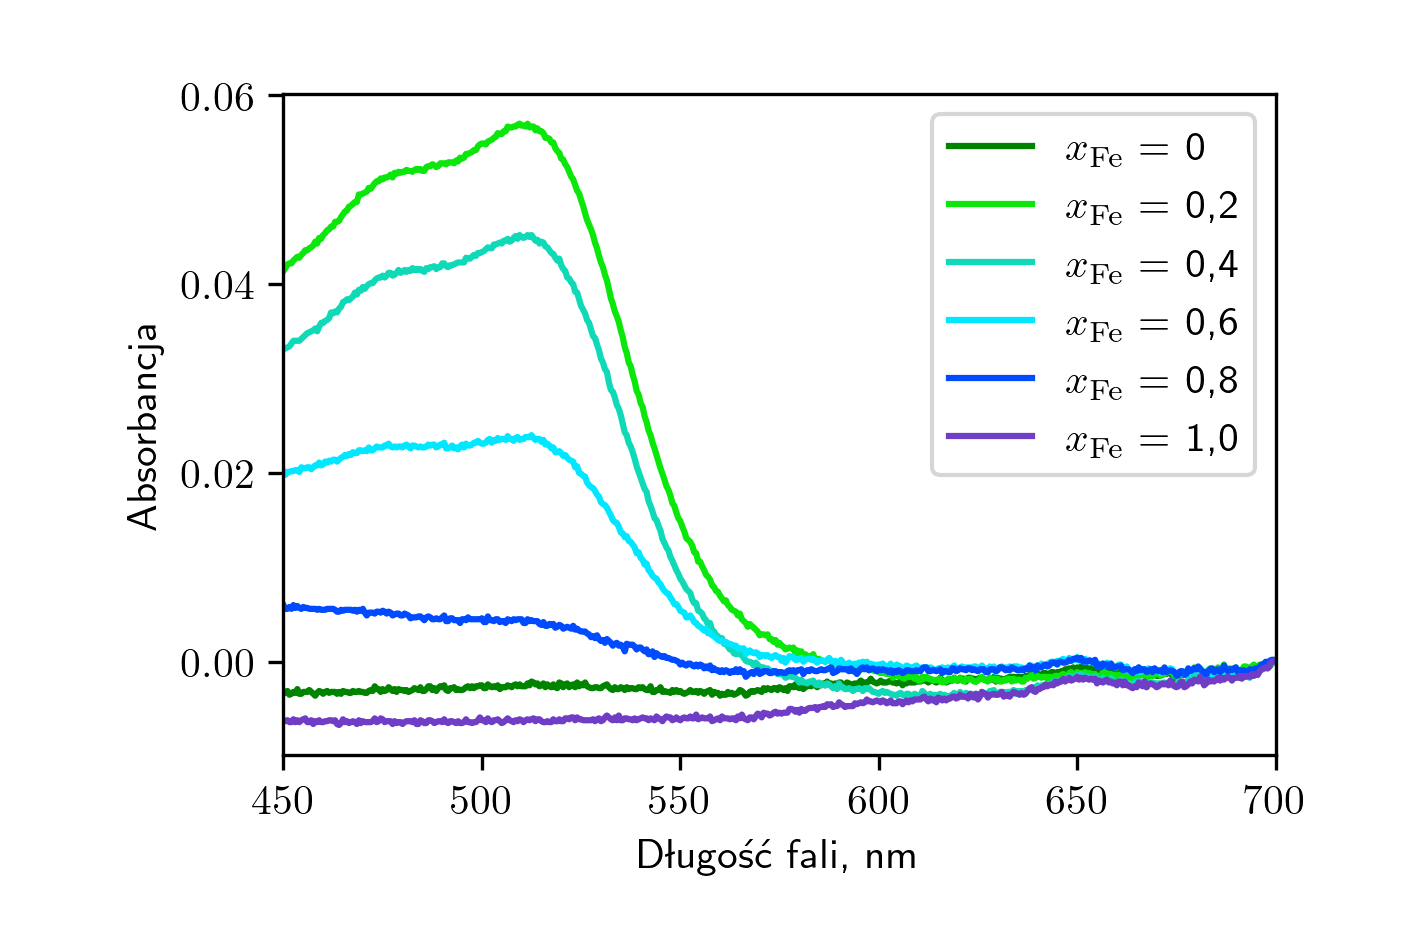
\includegraphics{ChFizLab_R3_widma1.png}
    \end{center}
    \caption{Widma absorbancji dla metody zmian ciągłych}
    \label{widma1}
\end{figure}


\noindent Wartości maksimum absorbancji dla widm poszczególnych roztworów zostały przedstawione na wykresie zależności od ułamka molowego jonów żelaza(II). Do punktów pomiarowych dopasowano dwie proste, które przecinają się dla $x_{\mathrm{Fe}} \approx$~0,22. Podczas dopasowywania prostej nie uwzględniono punktu dla $x_{\mathrm{Fe}}$ = 1,0, ponieważ odchylał się on od zależności liniowej. Wykres ten przedstawia Rysunek~\ref{AxFe}.


\begin{figure}[H]
    \begin{center}
        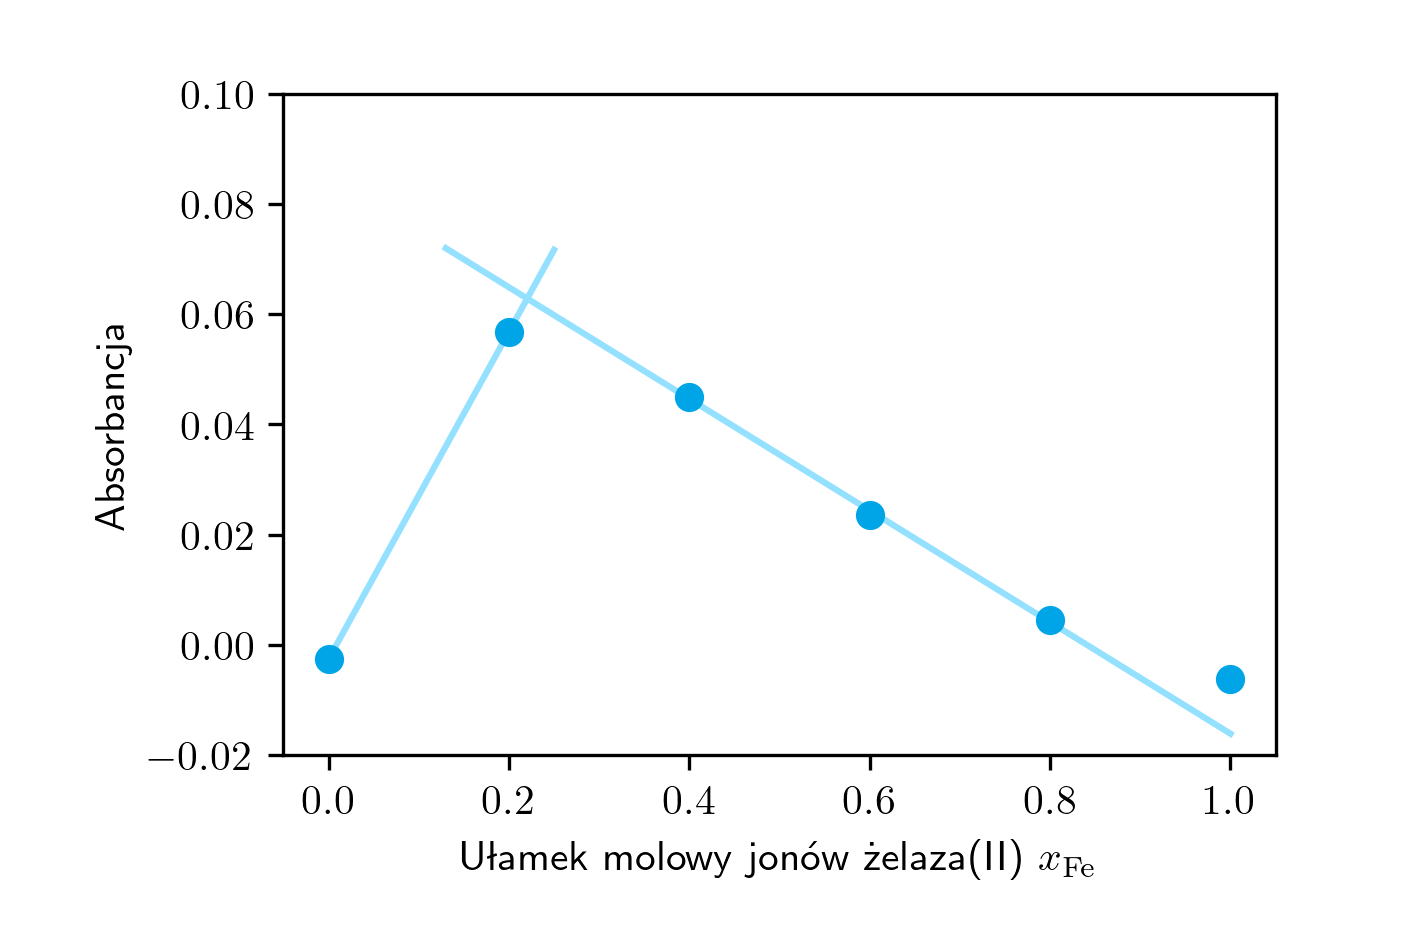
\includegraphics[height=7.5cm]{ChFizLab_R3_A(xFe).png}
    \end{center}
    \caption{Wykres zależności absorbancji dla długości fali 510~nm od ułamka molowego jonów żelaza(II)}
    \label{AxFe}
\end{figure}

Lewa dopasowana prosta jest opisana zależnością $A = 0,30 \cdot x_{\ce{Fe}}$, a~równanie opisujące prawą dopasowaną prostą to $A = -0,10 \cdot x_{\ce{Fe}} + 0,09$, gdzie $A$ to absorbancja. Współczynnik determinacji dopasowania prawej prostej jest równy 0,999.


\subsection{Metoda stosunków molowych}

Widma absorbancji roztworów wykonanych w~ramach metody stosunków molowych przedstawiono na Rysunku~\ref{widma2}.

\begin{figure}[H]
    \begin{center}
        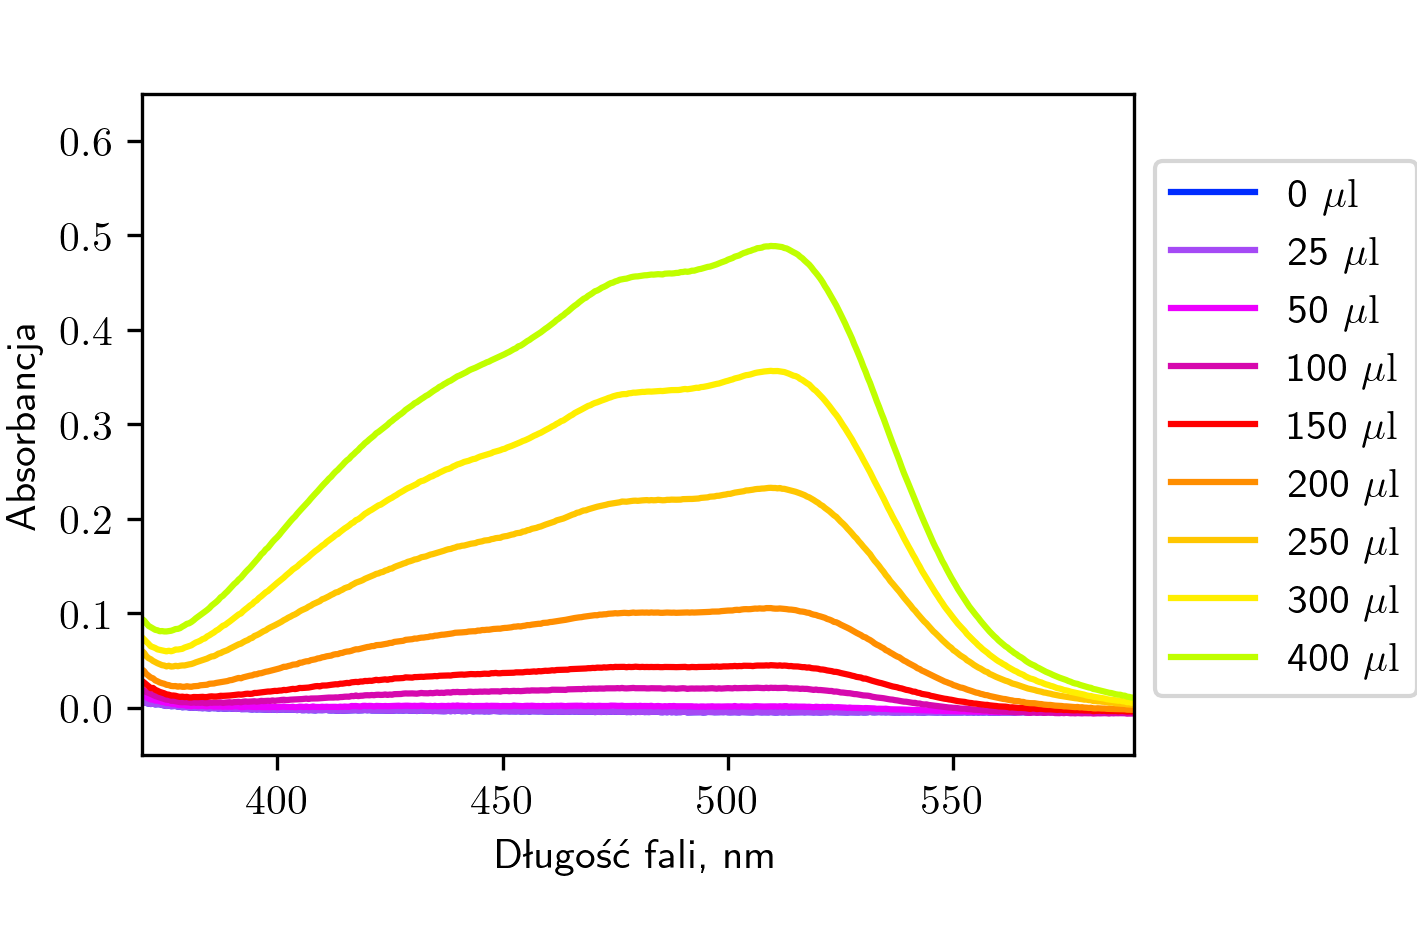
\includegraphics{ChFizLab_R3_widma2.png}
    \end{center}
    \caption{Widma absorbancji dla metody stosunków molowych}
    \label{widma2}
\end{figure}

\noindent Maksimum absorbancji również obserwowano dla długości fali 510~nm. Wartości absorbancji dla tej długości fali zostały przedstawione na wykresie w~zależności od stosunku $n_{\mathrm{fen}}/n_{\mathrm{Fe}}$ dla danego roztworu. Wykres ten przedstawiono na Rysunku~\ref{AnAnB}.

\begin{figure}[H]
    \begin{center}
        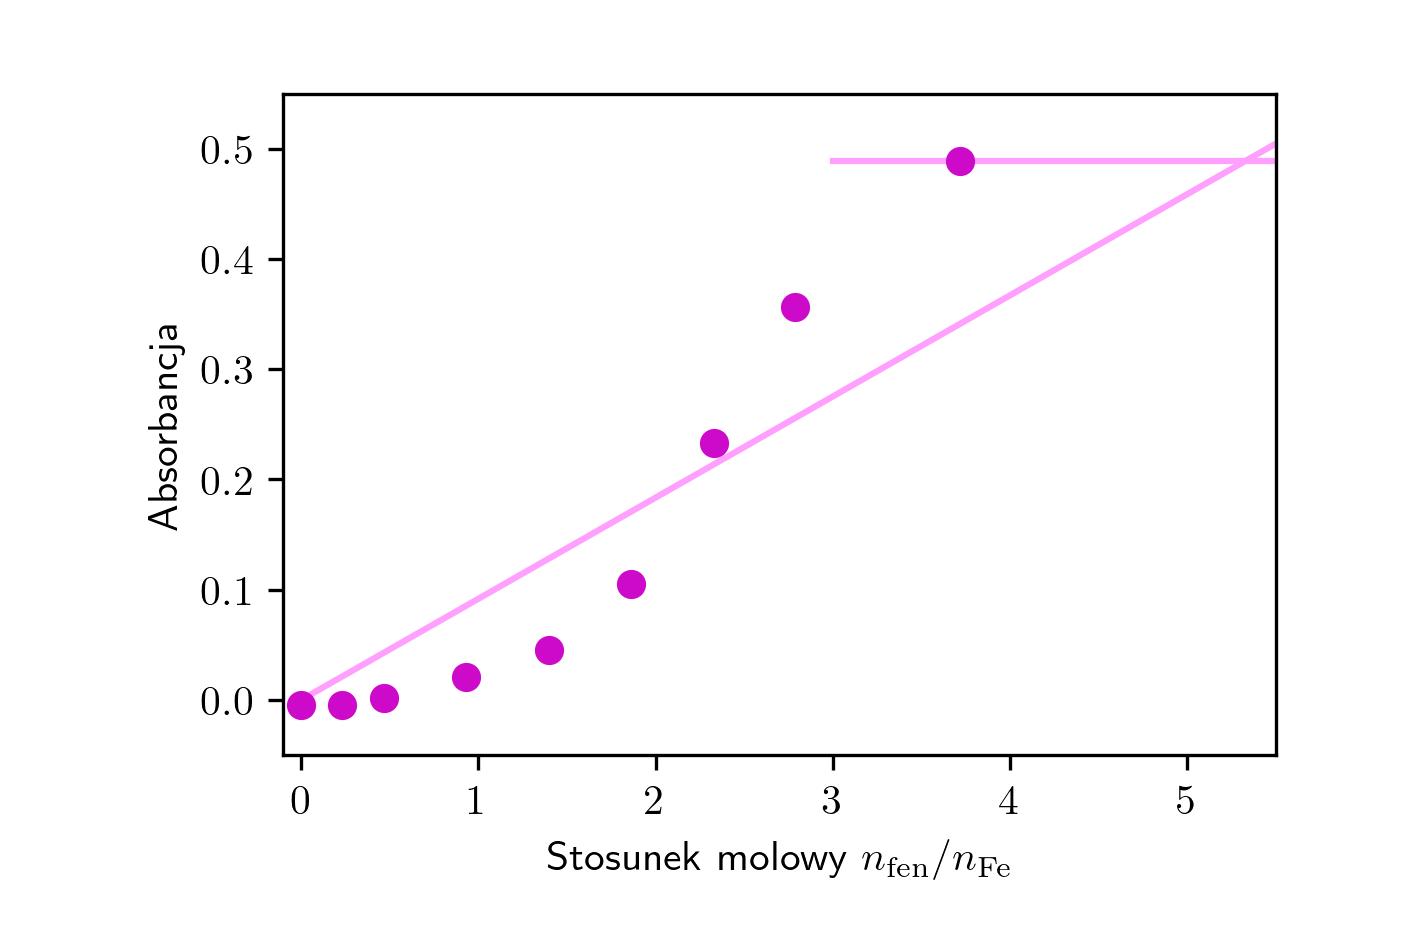
\includegraphics{ChFizLab_R3_A(nAnB).png}
    \end{center}
    \caption{Wykres zależności absorbancji od stosunku liczby moli $n_{\mathrm{fen}}/n_{\mathrm{Fe}}$}
    \label{AnAnB}
\end{figure}


Punkty pomiarowe 1--8, do których ma być dopasowana liniowa rosnąca zależność, nie układają się liniowo. Prosta dopasowana do nich jest opisana równaniem $A$ = 0,092$\cdot \frac{n_{\mathrm{fen}}}{n_{\mathrm{Fe}}}$ o~współczynniku determinacji równym 0,772. Proste przecinają się dla stosunku molowego równego 5,3.

Aby poprawić dopasowanie, zdecydowano się odrzucić niektóre punkty pomiarowe. Obecnie dopasowana prosta jest nachylona pod zbyt małym kątem, przecinając się z~drugą prostą z~prawej strony punktu pomiarowego dla roztworu po przekroczeniu stosunku stechiometrycznego. Z~tego względu zdecydowano się wykluczyć z~dopasowania punkty pomiarowe 1--5, które cechowały się zbyt małymi wartościami absorbancji. Pozostawiono punkty 6--8, otrzymując prostą opisaną równaniem $A$ = 0,270$\cdot \frac{n_{\mathrm{fen}}}{n_{\mathrm{Fe}}}$ - 0,397. Współczynnik dopasowania tej prostej wynosi 1,000.



\begin{figure}[H]
    \begin{center}
        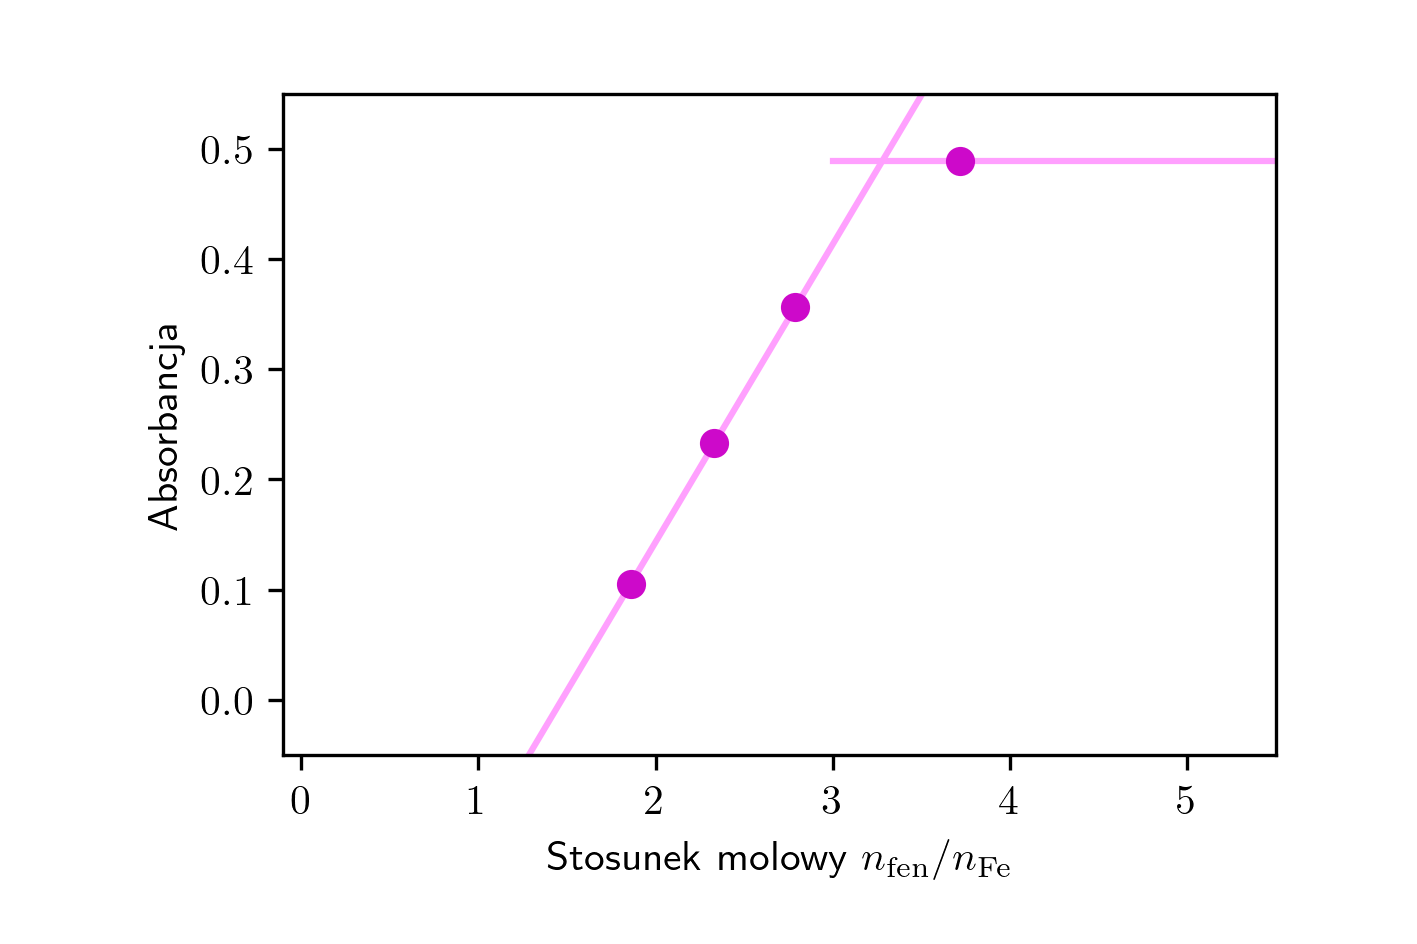
\includegraphics{ChFizLab_R3_A(nAnB)2.png}
    \end{center}
    \caption{Wykres zależności absorbancji od stosunku liczby moli $n_{\mathrm{fen}}/n_{\mathrm{Fe}}$ po selekcji punktów}
    \label{AnAnB2}
\end{figure}

Należy tu wspomnieć, że również prosta dla stałej wartości absorbancji wpływa na to, gdzie znajduje się punkt przecięcia. Ponadto, tylko jeden punkt decyduje tutaj o~wyznaczeniu tej prostej, co zmniejsza wiarygodność dopasowanego modelu.




\section{Dyskusja wyników}

 Kompleks utworzony przez jony żelaza(II) oraz \textit{o}-fenantrolinę to ferroina o~wzorze sumarycznym \ce{[Fe(fen)3]^2+} \cite{1}, zatem oczekiwany stosunek $n_{\mathrm{Fe}}$ do $n_{\mathrm{fen}}$ to 1:3.

% Metoda zmian ciągłych
Korzystając z równania (2) otrzymujemy, że ułamek molowy dla jonów żelaza(II) to 0,25. Wynik uzyskany eksperymentalnie to $x_{\mathrm{Fe}}$ = 0,22, co może wskazywać na stosunek składników kompleksu 1:4 (ułamek molowy byłby równy 0,20) lub 1:3 (wtedy ułamek molowy byłby równy 0,25). Otrzymane wyniki nie są zatem jednoznaczne, jednak wskazują również na stechiometrię zgodną z~faktyczną stechiometrią, czyli 1:3. Metoda zmian ciągłych umożliwiła zatem na wyznaczenie wartości zgodnych z~danymi literaturowymi.


% Metoda stosunków molowych
W przypadku metody stosunków molowych, punkty pomiarowe zależności absorbancji od stosunku molowego $\frac{n_{\mathrm{fen}}}{n_{\mathrm{Fe}}}$ nie cechują się liniowością (współczynnik determinacji równy 0,772). Fakt braku liniowości punktów pomiarowych może być spowodowany niedokładnie sporządzonymi roztworami, które w~rzeczywistości zawierały inne ilości \ce{Fe^2+} lub \textit{o}--fenantroliny. Być może niskie pH równe 2,40 wpływało niekorzystnie na tworzenie się kompleksu.

Do drugiego dopasowania prostej uwzględniono jedynie trzy punkty, tj. szósty, siódmy i~ósmy. Wyznaczone proste przecinają się dla stosunku molowego równego 3,28 $\approx$ 3, więc uzyskany wynik stechiometrii kompleksu to 1:3. Jest to wynik zgodny z~faktyczną stechiometrią kompleksu.

W~uzyskanych wynikach eksperymentalnych, istnieje tylko jeden punkt pomiarowy dla roztworu po przekroczeniu stosunku stechiometrycznego. Z~tego względu tylko ten jeden punkt decyduje o~wyznaczeniu prostej -- w~tym przypadku jest to możliwe, ponieważ jej współczynnik kierunkowy jest równy zeru. Jednakże, przeprowadzenie kilku pomiarów i~dopasowanie prostej do uzyskanych punktów pomiarowych umożliwiłoby uzyskanie bardziej wiarygodnego wyniku.

\begin{thebibliography}{9}
\bibitem{1}
R. K. Adhikamsetty, N. R. Gollapalli \emph{Complexation kinetics of \ce{Fe^2+} with 1,10-phenantroline forming ferroin in acidic solutions}, International Journal of Chemical Kinetics, 2008, str. 515--523
\end{thebibliography}





\end{document}

